\chapter{BACKGROUND}
This chapter is divided into four sections.  The first provides a general
introduction to the SOM algorithm and the problems created by using irregular
topology. The second reviews the current spherical topologies used with SOMs.
The third examines the flexibility of the various topologies with regard to
network size. The fourth takes a look at the limitations of using ``uniformity''
to evaluate potential topologies.

\section{Training and the Boundary Effect}
The SOM algorithm uses an artificial neural network to organize high-dimensional
data onto a low-dimensional lattice, or map, of neurons.  Each neuron contains a
reference vector that models the input data.  Before training, these
neuron-vectors are initialized, most commonly to random values.  During the
training process a randomly selected observation (input vector $x$) searches
all neurons (reference vectors $m_i$) to find the one to which it is most
similar, referred to as its Best Matching Unit (BMU $c$).  The BMU and its
neighborhood ($N_c$) are then adjusted to better match that observation
\citep{Kohonen2000}.  The training process is repeated a predefined number of
times, or ideally until the map converges.  The traditional SOM is laid out on a
two-dimensional plane using either a rectangular or hexagonal topology.
According to \cite{wu2006}, the hexagonal structure is more uniform and generally
preferred.

One drawback of building the neural lattice in a discrete Euclidean plane is the
boundary of the resulting lattice.  A neuron located on the boundary has fewer
neighbors and thus fewer chances of being updated \citep{wu2006}.  As observed
in Figure \ref{figure1}, neurons in the center of the map tend to better
represent the mean of the input-space.  This is arguably caused by outliers
being pushed to the edges of the map, where they encounter fewer competing
signals.
% Skupin's Comment here is not addressed.  Not sure if it needs a response or
% simply an acknowledgement.

\begin{figure}
\centering
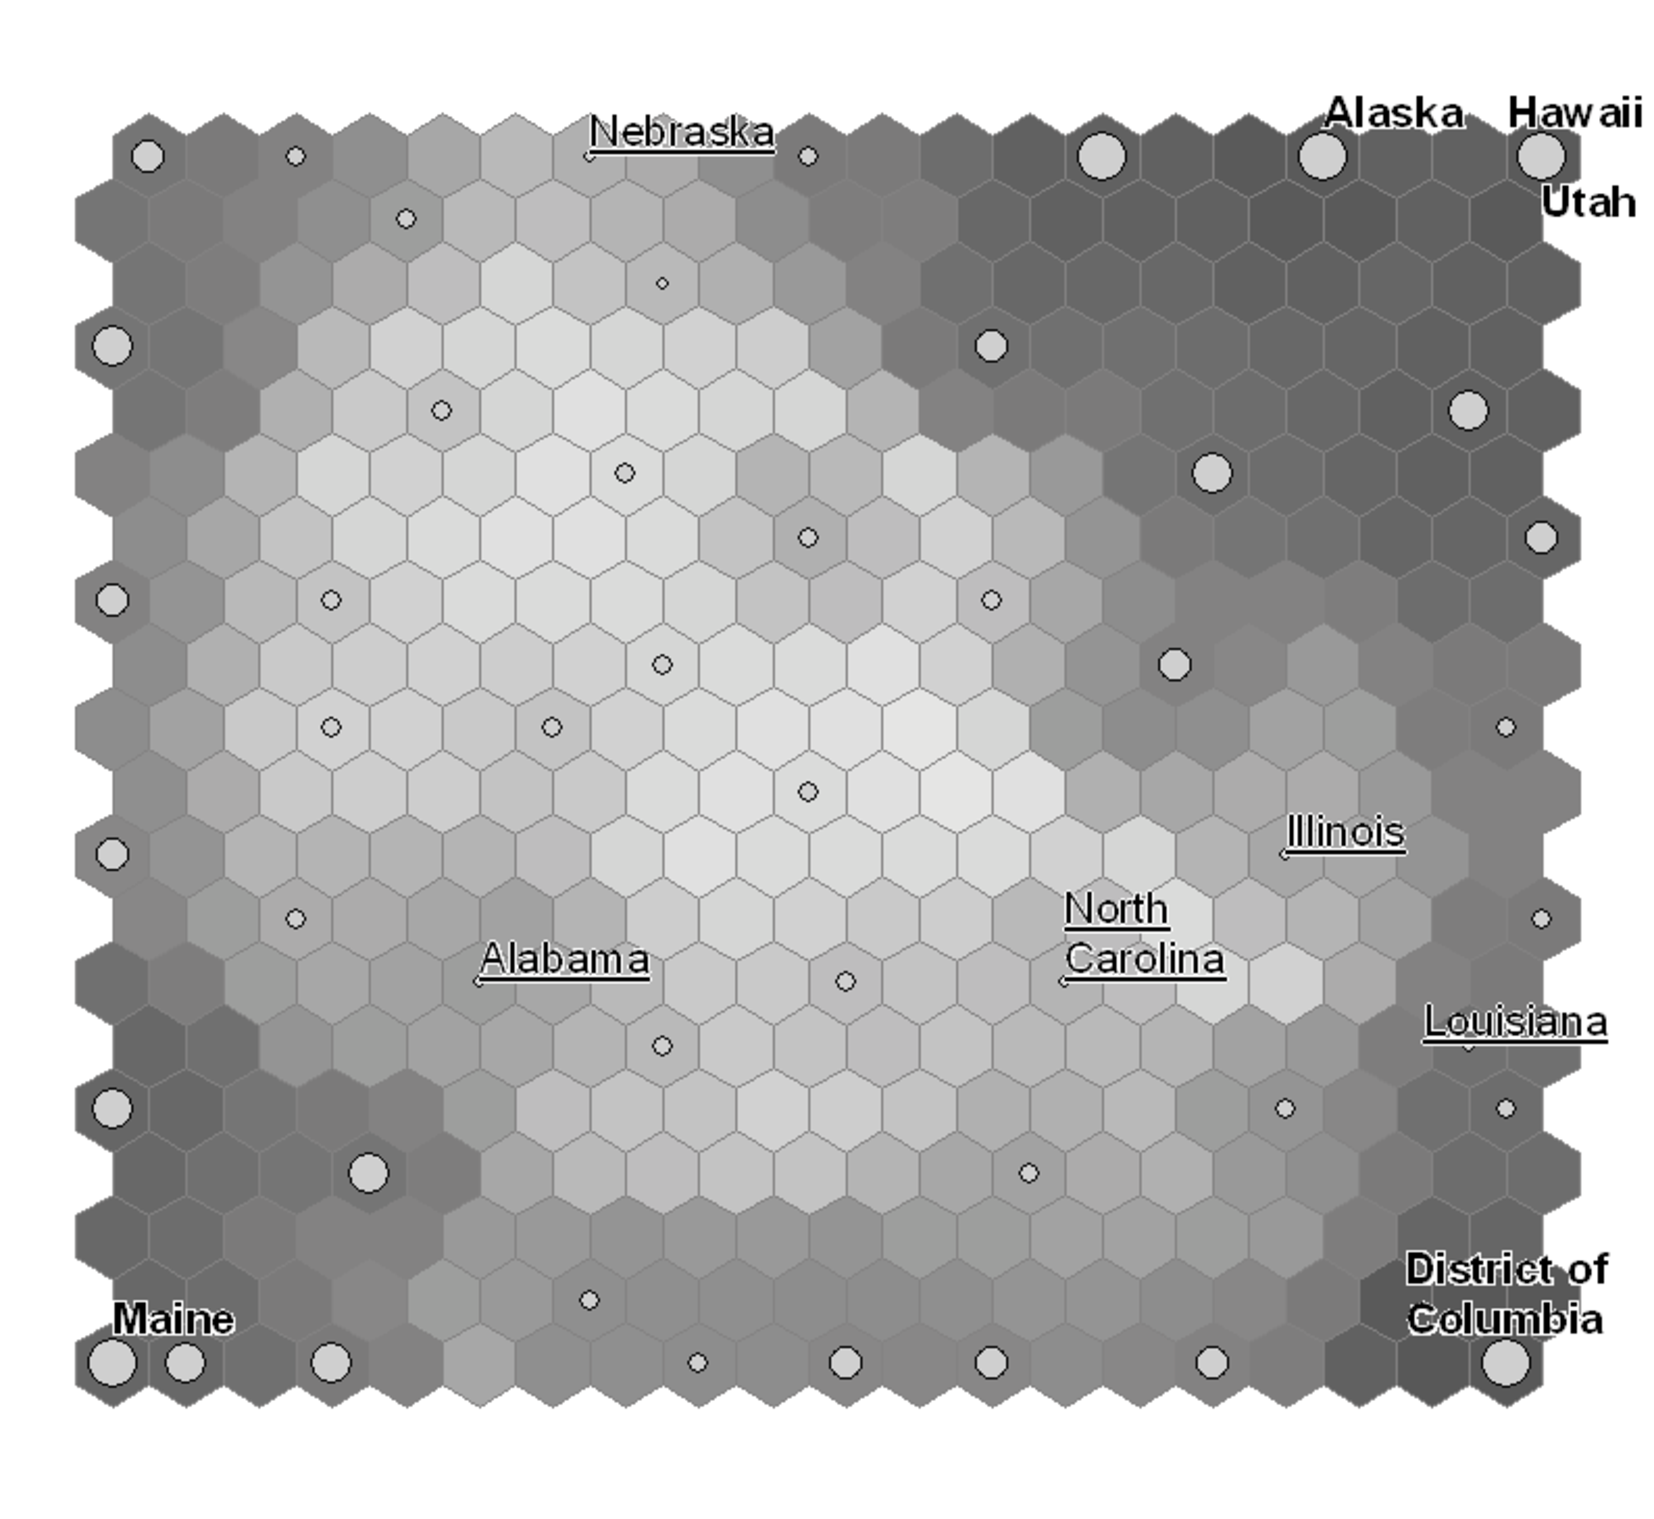
\includegraphics[width=\linewidth]{gridedge_grey.pdf}
\caption{Fifty States and the District of Columbia mapped onto a
SOM trained with thirty-two population census variables.  Darker neurons have a
relatively larger difference from the mean of the states, while lighter
neurons are relatively closer.  Smaller point symbols show states that are closer to the
mean, while large symbols show outliers. The five states closest to the average are shown
with underlined labels and the five states furthest from the mean are shown with
bold labels.}
\label{figure1}
\end{figure}

\section{Spherical SOM}
One way to eliminate the boundary effect is to wrap the lattice around a
three-dimensional object such as a sphere or torus, thereby removing the edge
entirely. The toroidal SOM was introduced by \cite{li1993}, however the torus is
not effective for visualization, as maps generated from a torus are not
very intuitive \citep{ito2000,wu2006}.  \cite{ritter99} describes the torus as
being topologically flat and suggests that a curved topology, such as that of a
sphere, may better reflect directional data.  A sphere also results in a more
intuitive map, since we are accustomed to looking at geographic maps based on a sphere.

\cite{ritter99} first introduced the spherical SOM, and several enhancements have
since been suggested \citep{boudjemai2003,sangole03,Nishio:2006fk,wu2006}.  A
good comparison of these enhancements can be found in \cite{wu2006}.  All of
these methods derive their spherical structure through the tessellation of a
polyhedron as originally proposed by \cite{ritter99}.  \cite{wu2006} point
out the importance of a uniform distribution on the sphere, and that it is
preferable for all neurons to have an equal number of neighbors and to be
equally spaced.  They find generally that the tessellation method best satisfies
these conditions, and specifically that the icosahedron is the best starting
point \citep{wu2005}. Tessellation of the icosahedron results in a network of
neurons, each of which having exactly six neighbors, save the original twelve
which each have five neighbors.  This is very close to the ideal structure in which every
neuron would have exactly six neighbors.  This structure has very low variances
in both neuron spacing and neighborhood size.

\section{Network Size}
\begin{figure}
\centering
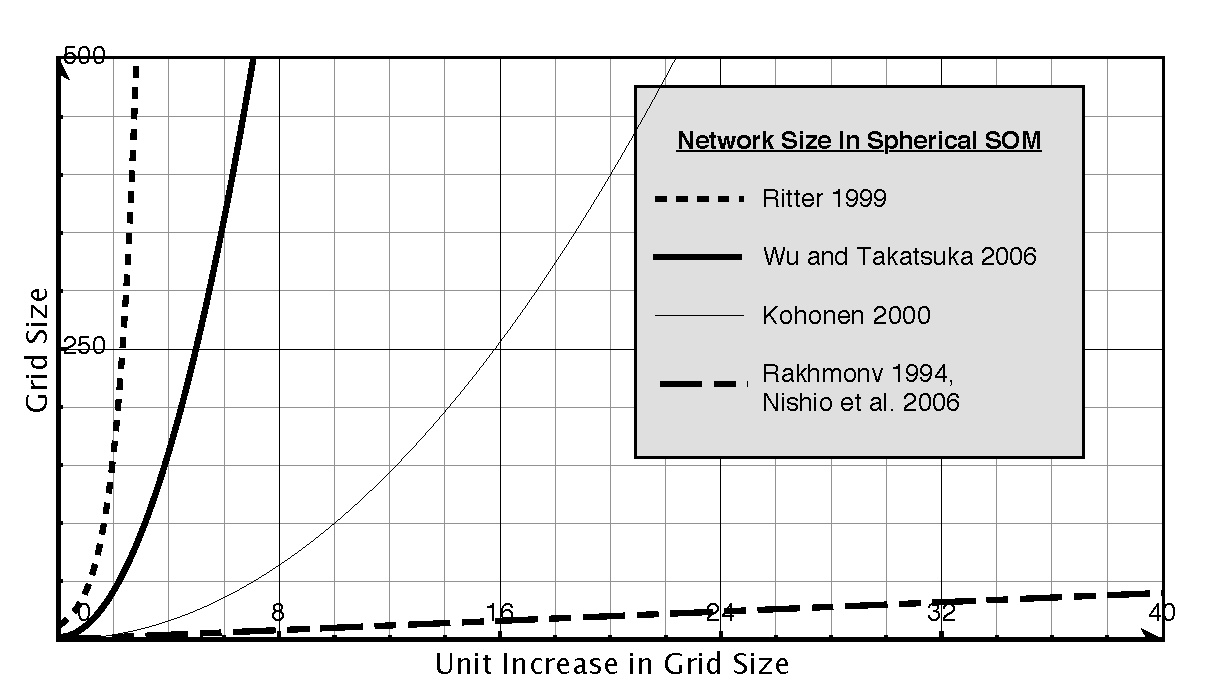
\includegraphics[width=\linewidth]{networkSize.pdf}
\caption{This figure demonstrates the achievable network size using various
spherical topologies, in comparison with the traditional SOM. The Y-axis represents the achievable network size, the
meaning of the X-axis is dependent on the topology. For the tessellation
methods the X-axis represents the frequency of the tessellation. For the
traditional Kohonen method the X-axis represents the size of both dimensions of
the grid; for comparability the ratio between the dimensions was fixed at one
($X_{dim}=Y_{dim}$).  For the \cite{Rakhmanov94} and \cite{Nishio:2006fk} methods the X-axis
represents the exact network size.}
\label{fig:nSize}
\end{figure}
The literature offers little theoretical guidance on choosing an appropriate
network size for a given dataset \citep{cho1996}.  \cite{toolbox} suggests
simply using a network size of \(5\sqrt {n}\), where \(n\) is the number of
observations. Given this lack of theoretical development, researchers should be
cautious when using methods that limit the control of network size.  Having a
high level of control over network size allows support for such very
different SOM applications as clustering versus low-dimensional spatial layout.
\cite{skupin07} demonstrate this when they use the same data to train two SOMs
of different sizes.  In the three-by-three (9) case the neurons act as
containers clustering similar states, while in the twenty-by-twenty (400) case
relationships are expressed with much finer granularity. As shown in
Figure \ref{fig:nSize}, methods for arranging an arbitrary number of points on a
sphere provide a much higher degree of flexibility when choosing a network
size.

The cost of relying on \citeauthor{ritter99}'s tessellation method is decreased
control over network size. \citeauthor{ritter99}'s tessellation method results
in a network size that grows at a rate of \(N=2+10*4^f\), where $f$ is the
frequency of tessellation. \cite{wu2006} offer a slight improvement. Rather than
recursively subdividing the faces, they redivide the original icosahedron with
each step, resulting in \(N=2+10*f^2\).  In practice, 2D Euclidean SOMs also offer
limited control over network size because it is undesirable to have one dimension
dramatically larger than the other. \cite{Nishio:2006fk} try to address the
issue of network size granularity by departing from the tessellation method and
suggesting the use of a partitioned helix to uniformly distribute any number of
neurons on a sphere.  A similar method proposed by \cite{Rakhmanov94} was
dismissed by \cite{wu2005} for failing to satisfy the uniformity conditions
described above.


\section{Uniformity}
\citeauthor{wu2006} state that ``[f]or SOM, it is desirable to have all neurons
receive equal geometrical treatment'' \cite[p. 900]{wu2006}.  To satisfy this
constraint, two conditions must be met.  First, each neuron should occupy the
same amount of space on the given surface.  Second, each neuron should be
bordered by the same number of surrounding neurons, and we should maximize that
number.  The first condition may be important for visualization, but is
irrelevant for training.  During the training of the SOM only the topology of
the neurons is considered.

Based solely on measures of neuron spacing, \cite{wu2005} dismissed a method
proposed by \cite{Rakhmanov94} for distributing points on a sphere.  Similarly
\cite{Nishio:2006fk} use these variance measures to support their helix
algorithm for distributing points on a sphere.  Table \ref{table1} shows that
these metrics can be misleading and comparison across topologies may not be
consistent.
The traditional rectangular and hexagonal topologies have no variance in neuron
spacing, and the generally preferred hexagonal structure displays greater
variance in neighborhood size than the rectangular structure.  The torus, by
comparison, would have variance in neuron spacing, yet no variance in
neighborhood size.  The distance between two neurons is only considered during
the formation of the neural network.  At this stage the spacing is significant
as it plays a part in determining neuron adjacency. However, using this measure
to evaluate potential topologies for use in SOM may be misleading.

\begin{table}[htbp]
\caption{Variances in Topologies}
\begin{center}
\begin{tabular}{|c|c|c|c|}
\hline
Topology&Grid Size&Neuron Spacing&Variance in Neighborhood Size\\
\hline
Rectangular&9x18&1&0.2716\\
Hexagonal&9x18&1&1.2138\\
Tessellation&162&0.25319 - 0.31287& 0.0686\\
Rakhmanov&162&0.15779 - 0.30069& 0.2908\\
\hline
\end{tabular}
\end{center}
\label{table1}
\end{table}

Methods for distributing points on the sphere, which allow for fine-grained
control over network size, produce slightly more irregular topologies.  However,
no substantive discussion of these irregularities or their effects on SOM
training exists in the literature. Given that limited theoretical guidance is available
for choosing network size, the desire for finer control over the network size
should not be overlooked. Particularly for larger SOMs, the desired network size
may not be achievable via tessellation of the icosahedron.

